%\chapter{Implementation Details}
 \chapter{Detalii de implementare}
\label{cap:implementare}


\section{Structura codului sursa}

Codul folosit pentru obtinerea sistemului \textit{\thesistitle} este impartit in 3 proiecte separate:
\begin{itemize}
	\item \textbf{Tor activity monitor} ce constituie logica necesara obtinerii listei de adrese IP blocate de sistem.
	\item \textbf{SQLi SVM} scopul acestuia fiind obtinerea modelului de SVM folosit pentru prevenirea atacurilor de SQL injection.
	\item \textbf{\thesistitle} reprezantand sistemul propus si incorporeaza rezultatele obtinute de celelalte doua proiecte.
\end{itemize}

\begin{figure}[h]
	\centering
	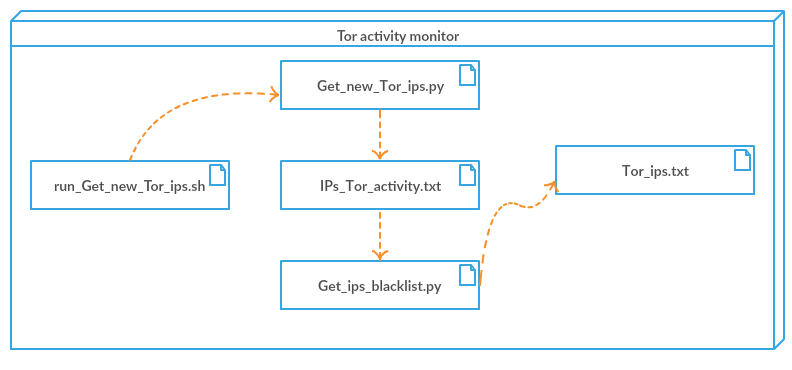
\includegraphics[width=0.8\textwidth]{tor_activity_monitor.png}
	\caption{Modulul pentru monitorizatea activitatii retelei Tor}
	\label{fig:tor_activity_monitor}
\end{figure}

Figura ~\ref{fig:tor_activity_monitor} prezinta care sunt fisierele folosite pentru monitorizarea activitatii retelei Tor si pentru obtinerea listei cu adresele IP ce trebuie blocate de catre sistem si relatiile dintre acestea. \\

\textbf{run\_Get\_new\_Tor\_ips.sh} este un fisier de bash ce are rolul de a rula Get\_new\_Tor\_ips.py. Fisierul este programat sa lanseze in executie Get\_new\_Tor\_ips.py la ore fixe, acesta ruland incontinuu pe un sistem cu acces la internet neintrerupt. Lnasarile in executie au loc o data la 6 ore, respectiv la ora 12 am si pm si 6 am si pm.

\textbf{Get\_new\_Tor\_ips.py} are rolul de a documenta modificarile de uptime din ultimele 6 ore ale nodurilor retelei Tor. Datele sunt furnizate de pe pagina "Tor Network Status" \cite{tot_status} si pentru fiecare adresa IP prezenta in date, se verifica care este uptime ul din ultimele 6 ore, informatiile acestea fiind stocate in IPs\_Tor\_activity.txt.

\textbf{IPs\_Tor\_activity.txt} are rolul de a stoca informatiile despre toate adresele IP utilizate de reteaua tor din ultima luna. Acestea sunt salvate in liste, pentru fiecare adresa IP in parte o lista. 

\textbf{Get\_ips\_blacklist.py} are rolul de genera fisierul Tor\_ips.txt folosit de catre sistemul propus pentru blocarea adreselor IP. Acesta foloseste datele din interiorul fisierului IPs\_Tor\_activity.txt, pentru a genera o lista cu toate adresele IP ce au un uptime total mai mare de 7 zile in ultimele 30 de zile.

\textbf{Tor\_ips.txt} reprezinta rezultatul proiectului. Acesta este alcatuit dintr-o lista formata din toate adresele IP ce vor fi blocate de sistemul propus in timpul rularii.

\newpage

\begin{figure}[h]
	\centering
	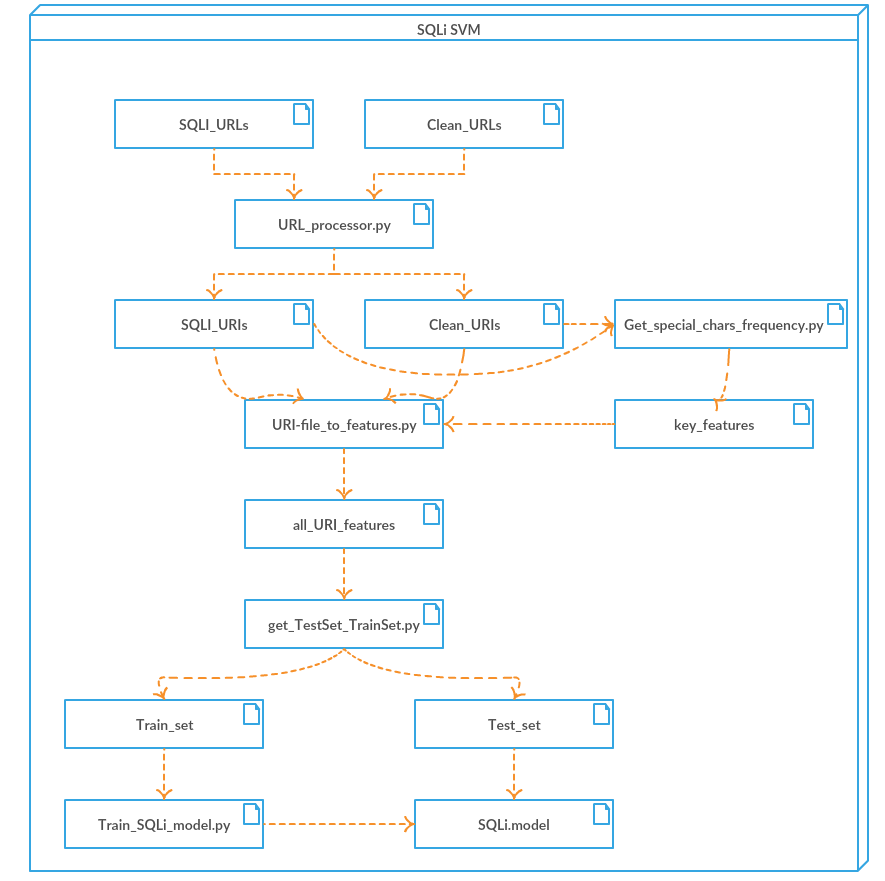
\includegraphics[width=0.8\textwidth]{sqli_svm.png}
	\caption{Modulul pentru prevenirea atacurilor SQL injection}
	\label{fig:sqli_svm}
\end{figure}
Figura ~\ref{fig:sqli_svm} prezinta care sunt fisierele utilizate pentru procesarea datelor necesare in procesul de antrenare a modelului de SVM, pana la obtinerea modelului propiu-zis si care sunt realtiile dintre acestea. \\

\textbf{SQLI\_URLs} reprezinta setul initial de date "infected" folosite pentru indentificarea atacurilor SQL injection. Acest set este constituit din URL-uri ce au fost indentificate de un produs autorizat ca fiind tentative de SQL injection.

\textbf{Clean\_URLs} reprezinta setul initial de date "clean" folosite pentru indentificarea atacurilor SQL injection. Acest set este constituit din URL-uri ce au fost indentificate de un produs autorizat ca fiind URL-uri curate.

\textbf{URL\_processor.py} primeste ca input un fisier sau string si are rolul de a procesa URL-uri intr-un format uniform(se elimina encodarile) si specific pentru pasii urmatori.

\textbf{SQLI\_URIs} constituie noua lista rezultata din procesarea fisierului SQLI\_URLs de catre URL\_processor.py.

\textbf{Clean\_URIs} constituie noua lista rezultata din procesarea fisierului Clean\_URLs de catre URL\_processor.py.

\textbf{Get\_secial\_chars\_frequency.py} are rolul de a caldula frecvventa de aparite a unor caractere speciale in cele doua seturi de date si de a decide in functie de frecventa lor de aparite, care din acestea sunt relevante in vederea alegerii trasaturilor de clasificare.

\textbf{key\_features} este o lista alcatuita din toate cuvintele cheie a limbajului SQL, dar si din caracterele speciale utilizate in acesta si considerate ca fiind relevante in urma executiei scriptului Get\_secial\_chars\_frequency.py.

\textbf{URI-file\_to\_features.py} are rolul de a procesa cele doua fisiere de date si pe baza trasaturilor din key\_features sa constituie un nou fisier ce contine pentru fiecare URL din cele doua fisiere tipul acestuia si trasaturile gasite in el, precum si frecventa lor.

\textbf{all\_URI\_features} este rezultatul rularii scriptului URI-file\_to\_features.py si contine pentru fiecare URL din cele doua fisiere de date, tipul acestuia si trasaturile gasite in el, precum si frecventa lor, acestea fiind folosite pentru antrenarea si testarea modelului de SVM.

\textbf{get\_TestSet\_TrainSet.py} are rolul de a 
imparti datele prezente in all\_URI\_features in doua seturi de proportie 70-30. Aceste doua seturi fiind folosite pentru antrenarea si testarea modelului.

\textbf{Train\_set} constituie 70\% din totalul de exemple acumulate pentru antrenarea modelului, doar acestea fiind de fapt folosite pentru antrenarea sa.

\textbf{Test\_set} constituie 30\% din exemplele acumulate, aceste date fiind folosite pentru testarea acuratetii modelului dupa antrenare.

\textbf{Train\_SQLi\_model.py} realizeaza obtinerea modelului de SVM folosit de sistem pentru prevenirea atacurilor SQL injection. Pentru antrenare modelului este folosit setul de date din fisierul Test\_set si algoritmi pusi la dispozitie de biblioteca open source libsvm \cite{libsvm}.

\textbf{SQLi.model} reprezinta rezultatul proiectului. Acesta este testat cu ajutorul setului de date din fisierul Test\_set si ulterior integrat in sistemul propus pentru a fi folosit pentru prevenirea atacurilo SQL injection.

\newpage

\begin{figure}[h]
	\centering
	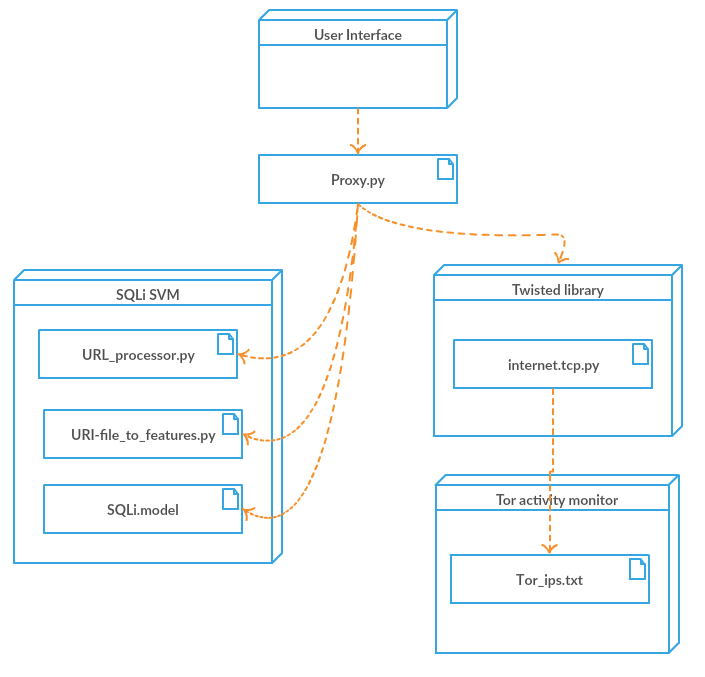
\includegraphics[width=0.8\textwidth]{source_code.png}
	\caption{Interactiunea dintre interfata grafica si celelalte module}
	\label{fig:source_code}
\end{figure}
Figura ~\ref{fig:source_code} prezinta care sunt fisierele, specific fiecarui modul, care sunt accesate in mod direct de catre interfata sau indirect de alte fisiere, in timpul rularii si relatiile dintre acestea. \\


\textbf{User Interface} reprezinta intreaga componenta ce realizeaza interfata de utilizator cu toate fisierele necesare realizarii ei, incorporate in compozitia sa. Aceasta a fost realizata de un proiect dezvoltat in .Net implicand multe fisiere cu scopul realizarii elementelor grafice. Aceste elementu nu vor fi tratate in aceasta sectiune.

\textbf{Proxy.py} reprezinta fisierul ce incorporeaza, respectiv leaga, tot codul ce constituie partea de "back end" a proiectului. In acest script de python se realizeara instantierea elementului de reverse proxy cu parametri de adrese IP si porturi aferente, precum si furnizarea metodelor de detectie componentei de reverse proxy.

\textbf{Twisted library} este o biblioteca open source scrisa in Python, ce ofera suport pentru diferite protocoale(TCP, UDP, SSL/TLS). Biblioteca a fost folosita pentru partea de cod ce ofera implementarea unui reverse proxy. Mare parte din fisierele oferite de acesta biblioteca au fost folosite fara a fi suprascrisa sau a li se aduce modificari ulterioare, insa in vederea atingeri scopului propus, asupra unor fisiere sursa au fost aduse mici modificari(internet.tcp.py).

\textbf{internet.tcp.py} este scriptul din biblioteca twisted ce ofera suportul pentru protocolul TCP. Acest fisiser a fost modificat pentru introducerea detectiei impotriva utilizatorilor de Tor. Script-ul integreaza lista realizata de proiectul "Tor activity monitor" pentru verificarea adresei utilizatorilor ce doresc sa stabileasca o conexiune TCP.




\section{Algoritmi, metode si API-uri}

In acesta sectiune se urmareste descrierea codului sursa folosit la realizarea sistemului propus si explicarea amanuntita a codului/metodelor considerate mai relevante, precum si a principalelor api-uri utilizate in implementarea acestuia. Abordarea codului sursa se realizeaza conform sub-proiectelor prezentate in sectiunea anterioara(Tor activity monitor, AQLi SVM, Interfata utilizator).

\subsection{Tor activity monitor}

Conform figurii ~\ref{fig:tor_activity_monitor}, acest proiect este realizat din 5 fisiere, acestea avand o relatie liniara intre ele.

Fisierul ce incepe ciclul de executie, run\_Get\_new\_Tor\_ips.sh, este un fisier de bash ce ruleaza in bucla infinta. Fisierul trebuie sa ruleze pe un sistem ce este functional non-stop si cu acces nelimitat la internet. La ore fixe acesta (12 am si pm si 6 am si pm), acesta lanseaza in executie scriptul de python Get\_new\_Tor\_ips.py.

Fisierul principal din acest proiect il reprezinta Get\_new\_Tor\_ips.py. Acesta descarca pagina "Tor Network Status" \cite{tot_status} si proceseaza datele de pe acestea, introducand in fisierul IPs\_Tor\_ activity.txt informatii referitoare la adresele IP gasite pe pagina si uptime-ul lor din ultimele 6 ore. Procesarea adreselor IP si extragerea valorii lor de uptime se poate observa in urmatoarele doua secvente de cod.

\lstset{language=python,frame=single, showstringspaces=false}
\begin{lstlisting}
time_up = row.findAll('td')[4].contents[0]
ip = row.findAll('td', attrs={'class':'iT'})[0].findAll('a',
 attrs={'class':'who'})[0].contents[0]


\end{lstlisting}

Pentru prelucrarea continutului paginii, acesta a fost downloadat in memoria programului, iar codul HTML rezultant a fost prelucrat cu ajutorul bibliotecii de python open source, BeautifulSoup. Codul de mai sus reprezinta extragerea valori de timp(uptime) si adresa IP careia aceasta corespunde. Variabila "row" fiind un elemnet din obiectul iterabil rezultat din initializarea bibliotecii BeautifulSoup cu codul HTML al paginii.

\lstset{language=python,frame=single, showstringspaces=false}
\begin{lstlisting}
days = time_up.split()[1]
if days == 'd':
    hours = 6
else:
    hours = int(time_up.split()[0])
    if hours > 6:
        hours = 6

\end{lstlisting}

In secventa de mai sus de cod, este indentificata valoarea corecta de uptime din ultimele 6 ore. Pentru cazul in care valoare de uptime este sub forma de zile sau aceasta este mai mare de 6 ore, ea se seteaza pe 6 ore, intrucat nu ne intereseaza decat activitatea din ultimele 6 ore.
\begin{lstlisting}
from bs4 import BeautifulSoup
from urllib.request import urlopen

pagesource = urlopen(page)
soup = BeautifulSoup(pagesource.read())
table = soup.findAll('table', attrs={'class': 'displayTable'})
\end{lstlisting}

Pentru procesarea continutului unei pagini web("Tor Network Status" \cite{tot_status}) s-au folosit bibliotecile de python, open source, urllib si BeautifulSoup \cite{btf_soup}. Biblioteca urllib ofera functii si clase ce pot fi folosite pentru deschiderea de URL-uri(urlopen). Functia folosita in codul de mai sus primeste ca parametru "page" adresa sub forma de string a paginii ce se doreste a fi citita. Biblioteca BeautifulSoup este o biblioteca de python folosita pentru extragerea de date din fisiere de HTML sau XML. Acesta este initializata cu un document HTML/XML si ca rezultat ofera un obiect ce permite navigarea prin codul sursa asemeni unei structuri de date imbricate. Astfel, spre exemplu, pentru indentificarea structurii corespunzatoare tabelei de adrese IP din codul sursa al paginii, s-a folosit o singura linie de cod, in care s-au specificat numele si atributele specifice acesteia.

Rezultatele rularii fisierului Get\_new\_Tor\_ips.py sunt actualizate in IPs\_Tor\_activity.txt. Acest fisier este de fapt un json in care se realizeaza dump la noul dictionar obtinut de  Get\_new\_Tor\_ips.py. Dictionarul este constituit din adresa IP ca si cheie si o liste .Structura acestor liste este realizata dintr-o serie de numere intre 0 si 6 ce reprezinta timpul total de uptime corespunzator sfertului respectiv de zi. Dimensiunea acestei liste este fixata la 30(zile)*4(sferturi de zi), pe masura ce un element nou este adaugat, primul element din lista fiind scos.

Urmatorul pas este filtrarea tuturor adreselor IP ce au un uptime mai mare de 7 zile. acest lucru este realizat de scriptul Get\_ips\_blacklist.py, iar rezultatele sunt stocate in Tor\_ips.txt, o adresa IP pe linie.

\subsection{SQLi SVM}
Desfasurarea proiectului incepe de la cele doua fisiere SQLi\_URLs si Clean\_URLs. In aceste doua fisiere se afla URL-uri complete din categoria conforma cu numele fiecarui fisier. Aceste fisiere sunt procesate de scriptul URI\_processor.py care are rolul de a uniformiza datele in aceasi encodare. Urmatoarea bucata de cod prezinta secventa ce transforma valorile hexa dintr-un URI in caractere si modul in care erorile de encodare sunt tratate(sunt printate pentru a fi tratate manual de catre programator):

\lstset{language=python,frame=single, showstringspaces=false}
\begin{lstlisting}
for index, sub_uri in enumerate(uri.split('%')):
    if sub_uri:
        if index == 0:
            new_uri = sub_uri
            continue
        try:
            hex_val = bytearray.fromhex(sub_uri[:2]).decode()
        except UnicodeDecodeError:
            print(uri + ' --- ' + sub_uri[:2])
            return ''
        new_uri += hex_val + sub_uri[2:]
\end{lstlisting}

Intrucat intr-un URL caracterul '\%' nu poate sa apara decat daca acesta este encodat('\%25'- valoarea pentru encodarea caracterului '\%'), indentificarea tuturor caracterelor encodate a fost facuta prin indentificarea tuturor caracterelor de tipul '\%' in URI. In cazul in care un astfel de caracter este gasit, se incearca conversia urmatoarelor doua caractere(asteptandu-se, conform conventiei, sa fie cifre), din valoarea in hexa corespunzatoare unui anumit caracter in caracterul in sine.


In urma procesarii datelor, rezulta cele doua fisiere SQLi\_URIs si Clean\_URIs, acestea avand acelasi continut cele anterioare insa in aceasi encodare. In urma obtinerii acestor doua fisiere, a fost realizata completarea listei de trasaturi(lista initiala este constituita din toate cuvintele cheie a limbajului SQL) cu caracterele speciale intalnite in acest limbaj. Scriptul Get\_secial\_chars\_frequency.py are rolul de a determina frecventa de aparitie a fiecarui caracter special in cele doua seturi de date, iar pe baza unei observatii umane, a fost realizata determinarea caracterelor ce constituie trasaturi rentabile. Urmatoarea bucata de cod este din scriptul Get\_secial\_chars\_frequency.py si realizeaza numararea URI-urilor(pentru comparare) din setul de date si frecventa caracterelor speciale("dict" este un dictionar cu cheile fiind caracterele speciale utilizate in limbaj):
\lstset{language=python,frame=single, showstringspaces=false}
\begin{lstlisting}
with open(args.f, 'r') as fd:
    for lines in fd.readlines():
        lines_nr += 1
        line = lines.strip()
        for keys in dict:
            if keys in line:
                dict[keys] += 1
                
\end{lstlisting}

Pentru indentificarea caracterelor relevante din limbajul SQL in comparatie cu cele folosite intr-un URL obijnuit, s-a ales numararea frecventei de aparitie a acestora in URL-uri normale, dar si in URL-uri ce contin atacuri de SQL injection. Numararea se face alternativ, rezultatele fiind furnizate ca doua seturi de date separate, bucata anterioara de cod reprezentand procesul doar pentru una dintre cele doua categorii. Dictionarul referit in cod este alcatuit dintr-un dictionar ce are ca si chei valoarea caracterelor specialae cautate, iar ca valoarea acestea sunt initializate pe zero pentru a fi incrementate o data cu numarul de aparitii ale caracterelor cautate. Pentru uniformizarea setului de date, intrucat distributia acestor caractere nu este tot timpul uniforma, se tine cont si de numarul de linii(pe fiecare linie se afla un URI distinct) in care au fost indentificate frecventele lor de aparitie.

Dupa determinarea caracterelor relevante, acestea au fost completate manual in fisierul key\_features, fisier ce insumeaza toate trasaturile ce sunt folosite in antrenarea modelului(fiecare linie contine o trasatura, numarul liniei fiind si indicele de referinta a trasaturii).

Pentru obtinerea datelor intr-un format ce poate fi procesat de biblioteca libsvm \cite{libsvm} a fost necesara transformarea acestora intr-un anumit format:

\begin{lstlisting}
+1 23:1 37:4 103:2
-1 54:1 77:1
\end{lstlisting}

Convertirea URI-urilor in formatul de mai sus este realizata de scriptul URI-file\_to\_features.py. Formatul de mai sus este reprezentarea fiecarui URL in functie de tipul acestuia si indicele trasaturii gasite in interiorul sau precum si frecventa de aparite a acestora(tip trasatura:frecventa trasatura:frecventa). Urmatoarele bucati de cod sunt extrasa din fisierul URI-file\_to\_features.py si realizeaza conversia unui URI in echivalentul sau in trasaturi:

\begin{lstlisting}
if keys in uri:
 if keywords_list.index(keys) > 184:
  keywords[keys] = uri.count(keys)
  if not uri.count(keys) == 0:
    ok = True
\end{lstlisting}

In lista cu trasaturi, primele 184 de pozitii corespund cuvintelor cheie ale limbajului SQL, urmatoarele 8 pozitii apartinand trasaturilor de tipul caracter special(determinate la pasul anterior de sciptul "Get\_special\_chars\_frequency.py"). In cazul in care o astfel de trasatura este gasita intr-un URI, pur si simplu se gaseste numarul total de aparitii a caracterului respectiv in URI.


\begin{lstlisting}
sub_uri = uri.split(keys)
for index, ele in enumerate(sub_uri):
  if index + 1 < len(sub_uri):
    if ele and sub_uri[index + 1] and not ele[-1].isalpha()
     and not sub_uri[index+1][0].isalpha():
      keywords_aux[keys] += 1
  elif not ele and sub_uri[index - 1]:
      keywords_aux[keys] += 1
\end{lstlisting}

Pentru trasaturile de pe primele 184 de pozitii, adica cuvintele cheie ale limbajului SQL, s-a abordat o logica mai complexa de procesre. O data ce un cuvant este gasit intr-un URI, pentru fiecare aparite a acestui cuvant se verifica ca primul caracter anterior cuvantului si primul urmator cuvantului sa nu fie litera, astfel eliminandu-se cazurile in care unele cuvinte sunt incluse in altele(ex: \textbf{all} si de\textbf{all}ocate).

In urma procesarii fisierelor de date, rezulta un fisier(all\_URI\_features) ce insumeaza toate datele utilizate in antrenarea modelului(exemple atat pozitive cat si negative), insa sub forma prezentata anterior(tip trasatura:frecventa trasatura:frecventa). Acest fisier este impartit in doua fisiere cu proportia de 70\% pentru Train\_set si 30\% Tes\_set de scriptul get\_Trainset\_Testset.py. cu scopul de a obtine un grup de date atat pentru antrenarea modelului cat si pentru testarea ulterioara a acestuia.

Pentru antrenarea modeluli, s-a folosit biblioteca open sourece libsvm. Aceasta biblioteca furnizeaza fisierele necesare antrenarii modelului de svm si de prezicere a unui rezultat pe un model existent. Apelul catre executabilul "svm-train.exe" se face prin intermediul scriptului de python Train\_SQLi\_model.py.
Executabilul de windows furnizat de biblioteca libsvm poate fi apelat conform exemplului urmator:

\begin{lstlisting} 
svm-train.exe [options] training_set_file [model_file]
\end{lstlisting}

\subsection{Interfata utilizator}

Componenta de interfata reprezinta atat proiectul in .net in care a fost realizata interfata sistemului, dar si fisierele/script-urile ce au rolul de a interconecta rezultatele celor doua proiecte anterioare cu acesta.

Scriptul Proxy.py incapsuleaza toate elemntele, din partea de back end, a proiectului propus. Acesta de asemenea furnizeaza ca output intr-un format specific(format ce este cunoscut si interpretat de interfata grafica) toate evenimentele ce apar in timpiul rularii sistemului. In acest script se realizeara instantierea elementului de reverse proxy cu parametri de adrese IP si porturi aferente, precum si furnizarea metodelor de detectie componentei de reverse proxy. Initializarea elementului de reverse proxy se realizeaza cu ajutorul codului oferit de biblioteca twisted. Acest cod este prezentat in "Anexa 1" a acestei lucrari.

In urmatoarele imagini sunt prezentate posibilele pagini ale interfatei utilizator precum si o scurta descriere ce ilustreaza functionalitatile oferite de paginile respective pentru utilizator.
\newpage]
 
\begin{figure}[h]
	\centering
	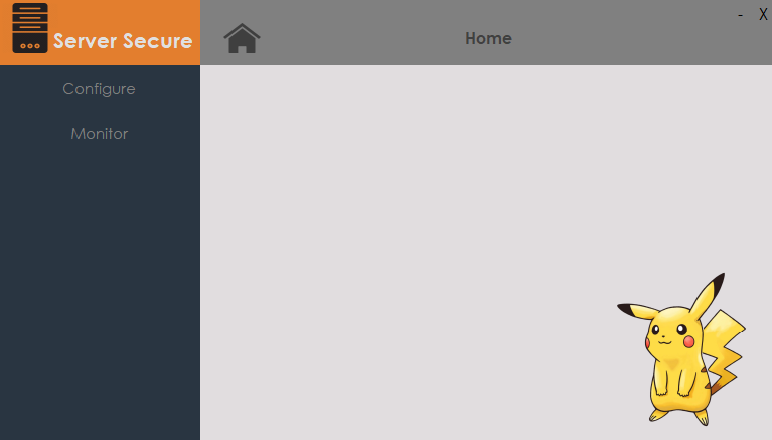
\includegraphics[width=0.6\textwidth]{ui_home.png}
	\caption{Meniul "Home" in interfata grafica}
	\label{fig:ui_home}
\end{figure}
Figura ~\ref{fig:ui_home} prezinta design-ul paginii de "Home" din interfata grafica pusa la dispozitie utilizatorilor sistemului. Acesta pagina este afisata la lansarea in executie a aplicatie, dar poate fi acesata de catre utlizator si prin apasarea butonului in forma de "casuta" din dreapta logoului aplicatiei.\\

\begin{figure}[h]
	\centering
	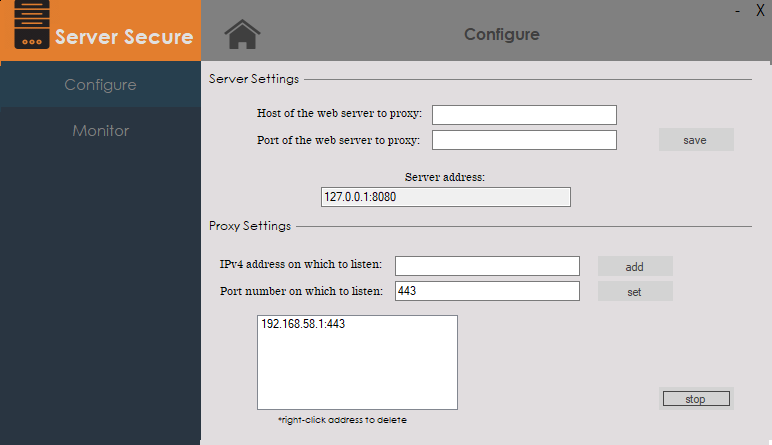
\includegraphics[width=0.7\textwidth]{ui_configure.png}
	\caption{Meniul "Configure" in interfata grafica}
	\label{fig:ui_configure}
\end{figure}
Figura ~\ref{fig:ui_configure} prezinta design-ul paginii de "Configure" din interfata grafica, in care utilizatorul sistemului poate sa seteze interfetele si porturile care vor fi tratate in timpul rularii. Partea superioara a meniului reprezinta setarile aferente partii de server, precum sugereaza si eticheta din stanga sus "Server Settings". In partea inferioara se pot seta detaliile interfetelor ce se pot conecta la server-ul setat mai sus.(aceste interfete pot fi multiple). \\

\begin{figure}[h]
	\centering
	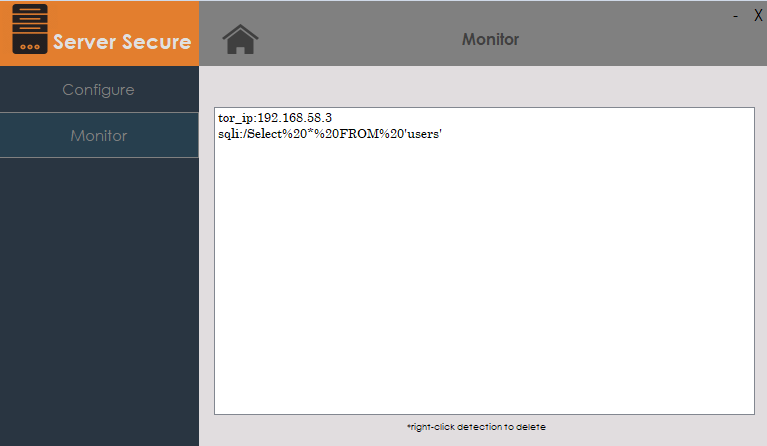
\includegraphics[width=0.8\textwidth]{ui_monitor.png}
	\caption{Meniul "Monitor" in interfata grafica}
	\label{fig:ui_monitor}
\end{figure}
Figura ~\ref{fig:ui_monitor} prezinta design-ul paginii de "Monitor" din interfata grafica, in care utilizatorul poate sa urmareasca activitatea sistemului in timpul rularii. In aceasta fereastra apar evenimentele aparute in timpul rularii aplicatiei, evenimente ce sunt sub forma de detectii.\\

\begin{figure}[h]
	\centering
	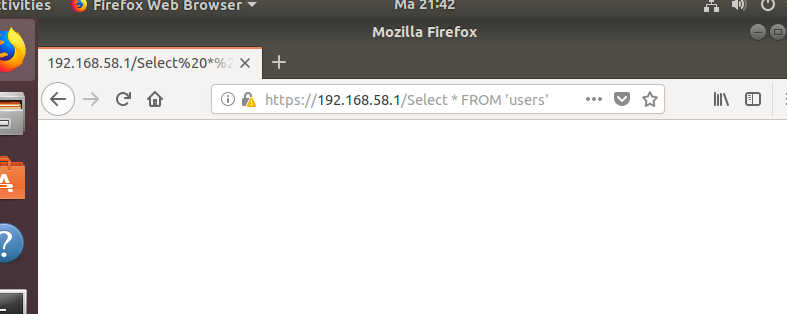
\includegraphics[width=0.9\textwidth]{sqli_respons.png}
	\caption{Raspunsul pentru SQL injection URL}
	\label{fig:sqli_respons}
\end{figure}

Figura ~\ref{fig:sqli_respons} prezinta cum arata raspunsul primit de la server de catre un utilizator dupa trimiterea unui request catre server, cu intentia de a realiza un atac de tipul SQL injection. Utilizatorului i se returneaza o pagina goala.\\
\newpage

\begin{figure}[h]
	\centering
	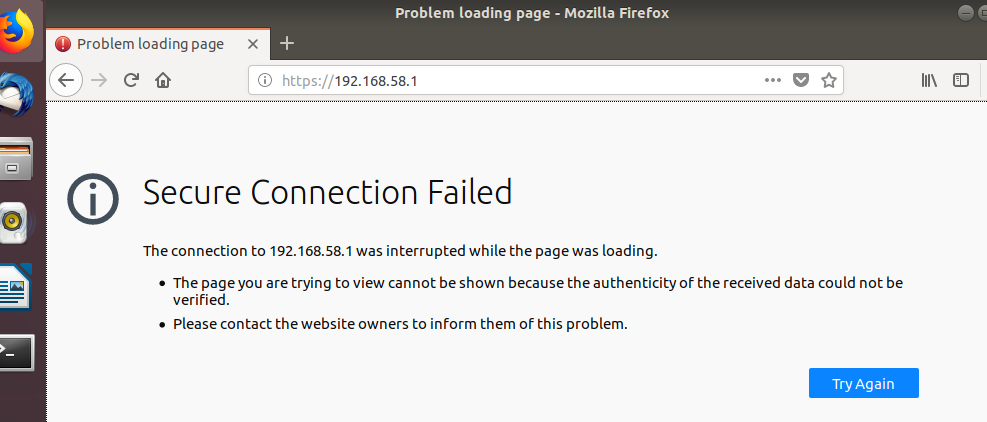
\includegraphics[width=0.8\textwidth]{tor_respons.png}
	\caption{Principalele module ale sitemului propus}
	\label{fig:tor_respons}
\end{figure}
Figura ~\ref{fig:tor_respons} prezinta cum arata raspunsul primit de la server de catre un utilizator al retelei Tor ce intentioneaza sa se conecteze la acesta. Acestor utilizatori li se refuza conexiunea. \\


%
%
%Conține detalii de implementare: 
%\begin{itemize}
%  \item organizarea codului sursă, organizarea logică a codului (module, ierarhii de clase)
%  \item descrierea claselor, funcțiilor, API-urilor importante ale aplicației
%  \item descrierea la nivel de implementare a algoritmilor principali
%  \item descrierea părților mai dificile
%  \item alte detalii de implementare relevante, specifice fiecărei aplicații
%\end{itemize}
%
%Descrierea implementării trebuie să reflecte modul în care ea corespunde (se mapează) design-ului. 
%
%Nu se vor da detalii irelevante. Descrierea codului trebuie gândită ca un ghid de parcurgere a codului sursă de către cineva care vrea să continue proiectul vostru. 
%
%Exemplu de cod:
%\lstset{language=C,frame=single, showstringspaces=false}
%\begin{lstlisting}
%# include <stdio.h>
%  
%int main (int argc, char **argv)
%{
%  int i;
%    
%  for (i=0; i<argc; i++)
%    printf("argv[%d] = %s\n", i, argv[i]);
%    
%  return 0;
%}
%\end{lstlisting}